This chapter presents an overview of the main works focused on the topics addressed in this dissertation.

\section{Related Works Description}
\label{s:RelatedWorks-Description}

The state-of-the art presents different computational techniques for data analysis, lots of works found in the \ac{WWT} field uses a combination of them to achieve their goal and improve the operation of the \acs{WWTP}s. Most of works aim to accomplish faults detection, control, soft-sensing, variable prediction, or just process understanding among others. Special attention will be given to the prediction task since it is the main focus of this investigation.
%either physical modelling, can have different purposes,

In \cite{Pang2019}, a q-learning (QL) algorithm with an activated sludge model (ASM2d-guided) reward setting was proposed. The integrated ASM2d-QL algorithms equipped with a self-learning mechanism were derived for optimizing the control strategies (hydraulic retention time (HRT) and internal recycling ratio (IRR)) of the WWTP system. In reference \cite{Li2013}, a Bayesian network-based approach was proposed for real-time prediction of a wastewater treatment system based on Modified Sequencing Batch Reactor (MSBR) . Based on the framework of the modified sequencing batch reactor prediction analysis, a Bayesian network model was constructed to analyze an MSBR using training data and information provided by domain experts.

Work \cite{Haggege2005} is a synthesis of a new neuro-fuzzy controller with an online learning procedure and a simple algebraic formulation, making it easy to interpret by a human being to control a bioreactor without requiring any analytical representation. The authors in \cite{Nadiri2018} focused on the Tabriz wastewater treatment plant (TWWTP), proposing an ensemble of fuzzy logic (FL), committee fuzzy logic (CFL)  and supervised CFL to predict water quality parameters. In \cite{Nourani2018}, three nonlinear models (feedforward neural network, adaptive neuro-fuzzy interference system and support vector machines (SVMs)) and a classical multilinear regression (MLR) were applied to predict the performance of the Nicosia wastewater treatment plant in terms of biochemical oxygen demand (BOD), COD and total nitrogen (TN). For paper \cite{Han2018}, a data-driven intelligent monitoring system was implemented (using the soft sensor technique and data distribution service). A fuzzy neural network (FNN) was applied for designing the soft sensor model.

The paper \cite{Guo2015} established two machine learning models—artificial neural networks (ANNs) and SVMs—to predict one-day interval TN concentration of effluent from a wastewater treatment plant in Ulsan, Korea. Reference \cite{Alsina2018} showed how machine learning models obtained better prediction results concerning traditional methods when increasing the size of the time-to-failure datasets. Four diverse machine learning approaches were implemented: ANN, SVM, random forest (RF) and soft computing methods. The reference \cite{Dairi2019} presented a data-driven anomaly detection approach based on deep learning methods and clustering algorithms to monitor influent conditions of WWTP, which affect treatment unit states, ongoing process mechanisms and product qualities. These techniques were recurrent neural networks (RNNs) and the function to delineate complex distributions from restricted Boltzmann machines (RBM), with various classifiers.

In work \cite{Bagheri2015}, multilayer perceptron ANN–genetic algorithm (MLPANN–GA) and radial basis function ANN–genetic algorithm (RBFANN–GA) models were successfully implemented for sludge volume index (SVI) prediction, taking into account that when sludge bulking appears, it causes poor settleability of sludge that results in poor effluent quality, loss of active biomass and increased costs and poses several environmental hazards. BOD, COD, nitrate, ammonia, TN, total phosphorus (TP), total suspended solids (TSS), total dissolved solids (TDS), mixed liquor volatile suspended solids (MLVSS ), mixed liquor suspended solids (MLSS), SVI, dissolved oxygen (DO), pH and T (Celsius) were measured and used for the estimation. The study \cite{Raduly2007} performed a simulation of plant behavior over a wide range of influent disturbances. An artificial neural network (ANN) was trained on the available WWTP, comparing ANN and a mechanistic WWTP model’s performances.

The study \cite{Liukkonen2013} proposed the Kohonen self-organizing map (SOM), a useful tool for illustrating the prevailing states of a process and their evolution, monitoring the alteration of wastewater quality and alerting in case of unusual behavior, such as increasing concentrations of harmful discharge components. The method provided an advanced and efficient way of monitoring and visualizing many measurements conducted in wastewater treatment. Article \cite{Jimenez2015} emphasized the high potential of some promising techniques, such as spectral analysis, and discussed issues that could appear soon concerning control of anaerobic digestion (AD) processes. The authors in work \cite{Reis2017} provided a critical outlook of the evolution of industrial process monitoring (IPM) since its introduction almost 100 years ago. Several evolution trends that have been structuring IPM developments over this extended period were briefly referred to, with more focus on data-driven approaches.

Work \cite{Zounemat-Kermani2019} is a survey of the feasibility of utilizing soft computing models in predicting emission factors (gaseous H2S) based on five input parameters, namely, the total dissolved sulfides, biochemical oxygen demand (BOD5), temperature, flow rate and pH. Multivariate nonlinear autoregressive exogenous (NARX) neural networks were developed and applied to predict weekly H2S in four WWTPs. The paper \cite{Yu2019} described an optimized extreme learning machine (ELM) based on an improved cuckoo search (ICS) algorithm for the design of the soft BOD measurement model.

Reference \cite{Ye2020} is a review of developments in artificial intelligence technologies for environmental pollution controls, including prediction of removal efficiency, evaluation of fuzzy logic to the control of the WWTP aerobic stage and AI-aided soft sensors for estimation of hard-to-measure variables. 
The study \cite{Hernandez-del-Olmo2019} performed different machine learning techniques to model a soft sensor to predict weather conditions such as SVMs, k-nearest neighbors (KNN), decision trees (DT), RFs and Gaussian naive Bayes (GND). With accurate weather prediction, an advanced control system can fit the parameters for better performance.

\section{Variable Prediction}
\label{s:RelatedWorks-variablePrediction}

One of the early approximations to intelligent monitoring and the predicting system was presented in \cite{Sanguesa2000} and \cite{Haggege2005}, where Bayesian networks and neuro-fuzzy logic were implemented to fulfill limitations of rule-based systems. Further works started to focus their attention on variable prediction using a variety of methods and a combination of them, taking the major advantages offered by each one. Reference \cite{Qin2012} used iterative predictor weighting–partial least squares (IPW–PLS) boosted by weighted predictions of a collection of regression models used as an ensemble prediction to estimate some water quality parameters. It was tested in the field, and its results showed a high correlation of the prediction. 

Several recent studies used fuzzy logic or neuro-fuzzy systems, such as \cite{Nourani2018,Nadiri2018,Han2018}, and some deep learning approaches, as in \cite{Guo2015,Alsina2018,Dairi2019}, which have provided high performance in prediction tasks. Studies like \cite{Bagheri2015} used a hybrid artificial neural networks–genetic algorithm approach to optimize the ANN estimation of the sludge bulking present in the sedimentation stage, which directly affects the effluent discharge water quality. Reference \cite{Dellana2009} made a performance comparison between the autoregressive integrated moving average (ARIMA) and time-delay neural network (TDNN) with such times-series variables as BOD and TSS and achieved more accurate predictions for real-world wastewater data with TDNN.

\section{Fault Detection}
\label{s:RelatedWorks-faultDetection}

There is a research branch whose aim is the opportune fault detection in very stringent processes, especially when it is part of the operational critical path where any unexpected event that occurs leads to a stagnation. Depending on the type of fault detection, the prediction of the problem can be focused on:
- The system’s ability to operate under some given circumstances.
- The time range in which equipment needs no maintenance and logistic support \cite{Alsina2018}.

Regarding system operability, faults and potential causes can be found before they occur by analyzing some patterns in WWTP data. The data visualization is capable of showing patterns that are products of a possible anomaly, known as abnormal patterns. These are classified as isolated, sustained, transient and drift \cite{Newhart2019}. Each one provides a hint about a future fault. Thus, it is possible to get fault information by looking at data behavior. Reference \cite{Dairi2019} implemented data-driven unsupervised anomaly detection approaches based on deep learning methods and clustering algorithms. The aim was to monitor and detect anomaly conditions in WWTP operations. The results showed its ability to detect the vast majority of abnormal events reported by the operator \cite{Dairi2019}. 

On the other hand, basic reliability analysis focuses on the prediction of the period in which equipment needs no support. This technique allows for finding a probability function R(t) to forecast the performance time of a component without failing until a given period t \cite{Alsina2018}. The work of \cite{Alsina2016} used an ANN to find the best cumulative failure distribution of mechanical components, which had a performance to fit a set of failure data and estimate its parameters, especially under poor data conditions. As a result, the networks with a momentum equal to 0.75 produced the best approximation 83.46\% of the time \cite{Alsina2016}.



\begin{figure}[t]
\centering
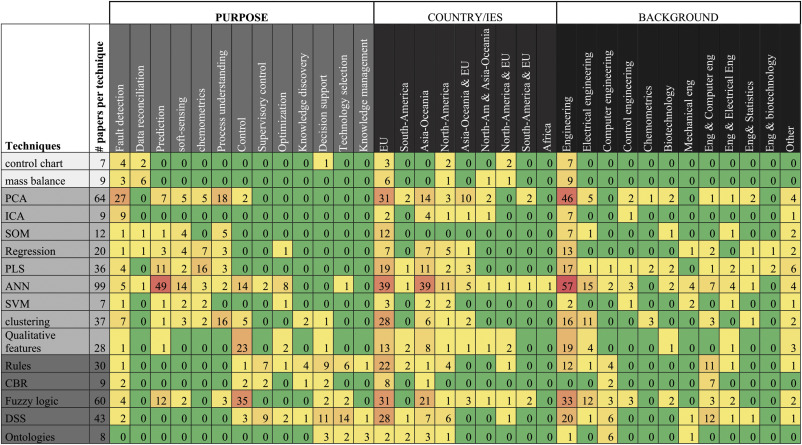
\includegraphics[width=16cm]{tables/PaperTable.jpg}
\caption{Number of papers per technique, for different purposes (only the main purpose of the method for each paper was considered), regions and background from the authors of the publications.}
\label{f:Papers Table}
\end{figure}


\section{Summary}
\label{s:Related-Works-Summary}

The final section of each major chapter should summarize the chapter. In comparison to the chapter, the summary should be short ($\frac{1}{2}$ to $2$ pages is normal).
